\chapter{MIP Timing Detector (MTD)}
\section{Introduction}

In the coming years the LHC will be working toward upgrades that will lead a substantial increase in luminosity.  The timeline for future operations of the LHC is shown in Figure \ref{fig:lhctimeline}.  In 2019 the LHC entered a two-year shutdown, Long Shutdown 2 (LS2).  Upgrades of the LHC injector complex to increase the beam brightness will take place during this shutdown.  After LS2 the LHC will enter Run 3 which will run for three years at 13-14 TeV.  At the completion of Run 3 the LHC will enter Long Shutdown 3 (LS3) which will last approximately 2.5 years.  During LS3 the optics in the interaction region will be upgraded to produce smaller beams at the interaction point.  The completion of this upgrade will usher in the High Luminosity (HL-LHC) era or Phase 2 of LHC operations, during which the combination of brighter beams and a new focusing scheme at the IP allows for a potential luminosity of 2x10$^{35}$ cm$^{-2}$s$^{-1}$ at the beginning of each fill \cite{Apollinari:2017cqg}.  

\begin{figure}[h]
	\centering
	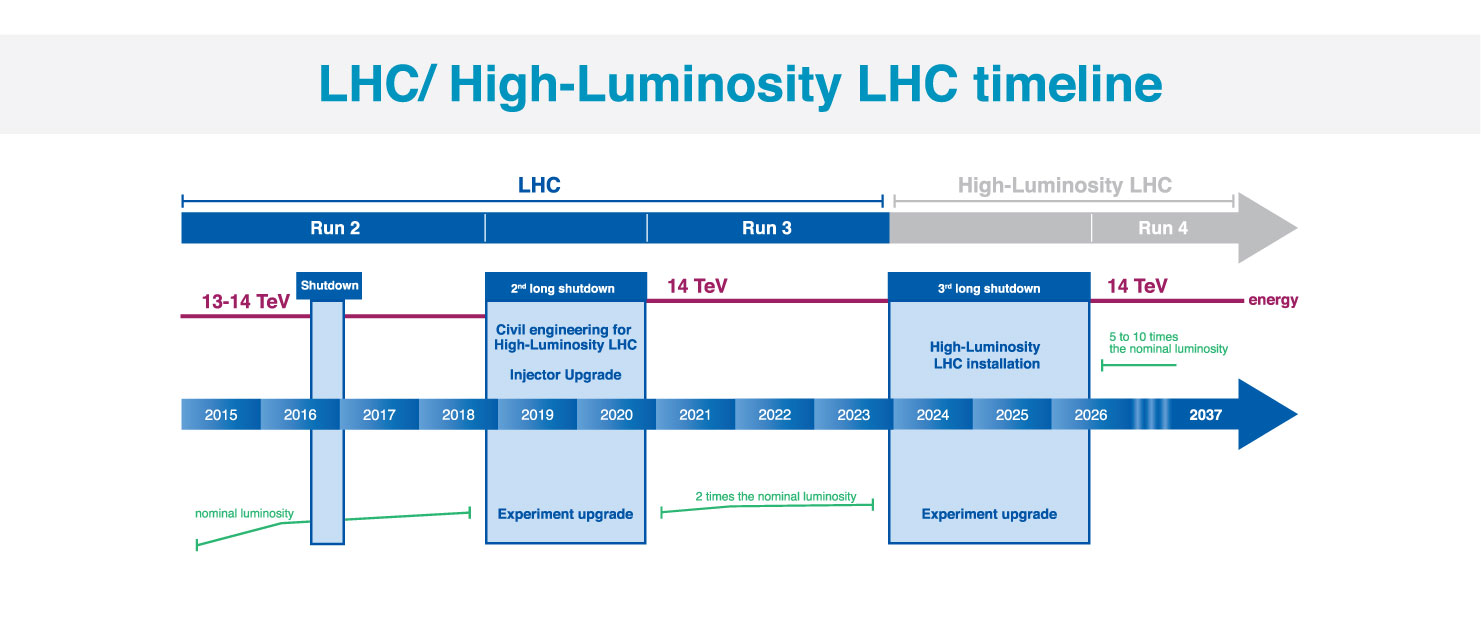
\includegraphics[width=1.0\linewidth]{Figures/LHCTimeline}
	\caption[Timeline for LHC]{Timeline for LHC \cite{DeMelis:2063307}}
	\label{fig:lhctimeline}
\end{figure}

The increased luminosity results in more interactions per bunch crossing or pileup.  In order to limit the amount of pileup the experiments must disentangle to more manageable levels, the nominal scenario would be operating at a stable luminosity of $5.0\times10^{34}$ cm$^{-2}$ s$^{-1}$.  This would limit the pileup to an average of 140.  The ultimate scenario for operations would be running at $7.5\times10^{34}$ cm$^{-2}$ s$^{-1}$ which brings the average pileup up to 200.  The CMS detector in its current state is not capable of dealing with $\approx$140-200 pileup.  At this level of pileup the spacial overlaps of tracks and energy depositions would lead to a degradation in the ability to identify and reconstruct hard interactions. In order to preserve the data quality of the current CMS detector this increased pileup must be reduced to an equivalent level approximately equal to current LHC operations which is $\sim$40.  The collision vertices within a bunch crossing have an RMS spread of 180-200 ps in time.  If the beam spot were to be sliced into consecutive snap shots of 30-40 ps then the pileup levels per snapshot would be approximately 40.  The space-time reconstruction of a 200 pileup event is shown in Figure \ref{fig:pileup4d}.  The addition of timing information to the $z$ position spreads apart the vertices that would otherwise have been merged together and indiscernible.  In order to achieve this a detector dedicated to the precise timing of minimum ionizing particles (MIPs), the MTD, will be added to the CMS detector.



\begin{figure}[h]
	\centering
	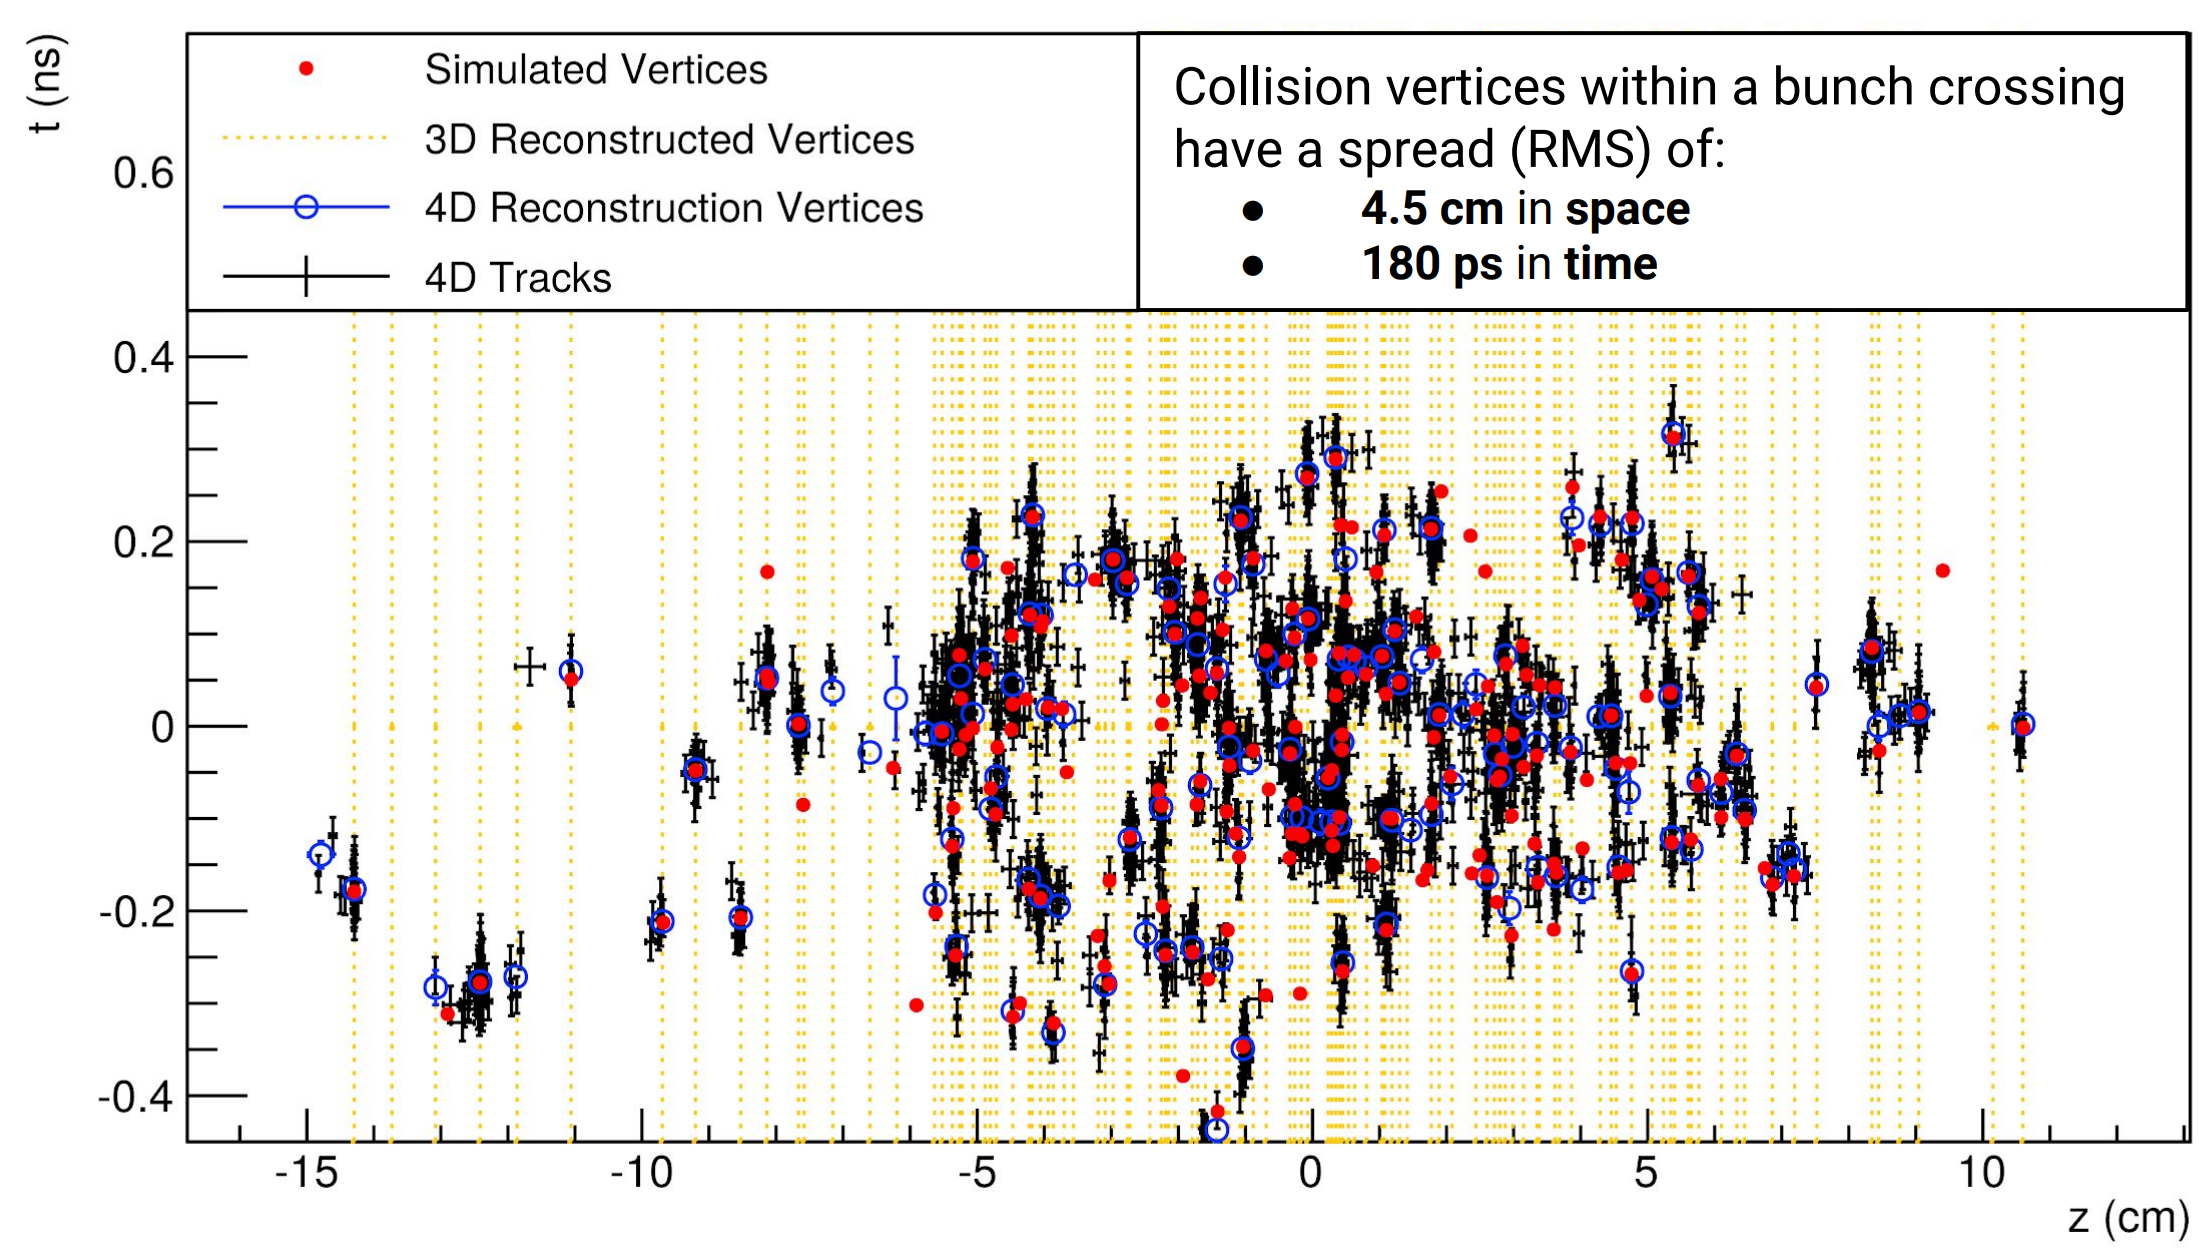
\includegraphics[width=0.7\linewidth]{Figures/Pileup_4D}
	\caption{Vertices from a simulated 200 pileup event.  Need to replace this with the figure from the TDR. }
	\label{fig:pileup4d}
\end{figure}



%The MTD will provide timing information with a resolution of 30-40 ps at the start of the HL-LHC era.  Radiation damage is expected to degrade this to 50-60 ps by the end of the HL-LHC era.


\section{Barrel Timing Layer}
 The Barrel Timing Layer (BTL) makes up the barrel region of the MTD.  It will provide pseudorapidity coverage up to $|\eta| = 1.48$ with a geometric acceptance of $\sim 90\%$.  The BTL will be capable of detecting MIPs with a time resolution of 30 ps at the start of Phase-2 operations and a luminosity-weighted time resolution of $\sim45$ ps when radiation damage effects are taken into account.


